\documentclass[a4paper,11pt]{report}
\usepackage[showexo=true,showcorr=false]{../packages/coursclasse}
%Commenter ou enlever le commentaire sur la ligne suivante pour montrer le niveau
\toggletrue{montrerNiveaux}

%\usepackage{cmbright}
\usepackage{arev}
\usepackage{enumitem}
\setlist[enumerate]{align=left,leftmargin=1cm,itemsep=10pt,parsep=0pt,topsep=0pt,rightmargin=0.5cm}
\setlist[itemize]{align=left,labelsep=1em,leftmargin=*,itemsep=0pt,parsep=0pt,topsep=0pt,rightmargin=0cm}

\setlength\columnsep{35pt}

\usepackage{mathrsfs}
\usetikzlibrary{arrows}
\begin{document}


%%%%%%%%%%%%%%%%% À MODIFIER POUR CHAQUE SERIE %%%%%%%%%%%%%%%%%%%%%%%%%%%%%
\newcommand{\chapterName}{Espace}
\newcommand{\serieName}{Points, segments, droites}


%%%%%%%%%%%%%%%%%% PREMIERE PAGE NE PAS MODIFER %%%%%%%%%%%%%%%%%%%%%%%%
% le chapitre en cours, ne pas changer au cours d'une série
\chapter*{\chapterName}
\thispagestyle{empty}

%%%%% LISTE AIDE MEMOIRE %%%%%%
\begin{amL}{\serieName}{
\item Définition et notation de la droite (page 90)
\item Définition et notation de la demi- droite (page 90)
\item Définition et notation du segment (page 90)
\item Distance (page 91)
\item Droites sécantes (page 92)
\item Droites perpendiculaires (page 93)
\item Droites parallèles (page 94)
}
\end{amL}

%%%%%%%%%%%%%%% DEBUT DE LA SERIE NE PAS MODIFIER %%%%%%%%%%%%%%%%%%%%%%%%%%%%%
\section*{\serieName}
\setcounter{page}{1}
\thispagestyle{firstPage}


%%%%%%%%%%% LES EXERCICES %%%%%%%%%%%%%%%%%%%%%%%%%%%%%%%%%%%%

\begin{QSJ}{103}{1}
\end{QSJ}



\begin{resolu}{Notation et vocabulaire} {Complète les consignes suivantes par les mots ou symboles qui conviennent, puis effectue les constructions nécessaires: 
\begin{tasks}(2)
\task Trace la droite $(AB)$.
\task Trace la demi-droite $[CD)$.
\task Trace le segment $[AC]$.
\end{tasks}
\begin{center}
\includegraphics[scale=0.8]{media/es-11/13-r1}
%\psset{xunit=1cm,yunit=1cm,algebraic=true,dimen=middle,dotstyle=o,dotsize=5pt 0,linewidth=2pt,arrowsize=3pt 2,arrowinset=0.25}
%\begin{pspicture*}(-3.679241373890801,-2.5414930385785395)(2.094367811575665,4.627174825672888)
%\psplot[linewidth=2pt,linecolor=blue]{-3.679241373890801}{2.094367811575665}{(--1.5581077617604557-3.0939915252260493*x)/2.5000556520799773}
%\psplot[linewidth=2pt,linecolor=blue]{-2.2427453086072777}{2.094367811575665}{(-3.7027657711479147-1.2707465192892702*x)/2.05805686276197}
%\begin{scriptsize}
%\psdots[dotstyle=x](-1.4830598894669533,2.4586182655814164)
%\rput[bl](-1.427810040802203,2.5967428872432934){$A$}
%\psdots[dotstyle=x](1.016995762613024,-0.6353732596446328)
%\rput[bl](1.0722456112777738,-0.4972486379827564){$B$}
%\psdots[dotstyle=x](-2.2427453086072777,-0.4143738649856292)
%\rput[bl](-2.1874954599425274,-0.2762492433237529){$C$}
%\psdots[dotstyle=x](-0.18468844584530772,-1.6851203842748994)
%\rput[bl](-0.1294385971805576,-1.5469957626130233){$D$}
%\end{scriptsize}
%\end{pspicture*}
\end{center}
}
{1}
\end{resolu}

%\begin{exop}
%{Complète les consignes suivantes par les mots ou symboles qui conviennent:
%\begin{tasks}
%\task Trace \ligne{4} $[AB)$.
%\task Trace \ligne{4} $[CD]$.
%\task Trace \ligne{4} $(EF)$.
%\task Trace la droite \ligne{1} GH \ligne{1}.
%\task Trace la demi-droite \ligne{1} IJ \ligne{1}.
%\task Trace le segment \ligne{1} KL \ligne{1}.
%\end{tasks}
%}
%{1}
%\end{exop}

\begin{exop}{Trace
		\vspace{-0.3cm}
\begin{tasks}[after-item-skip = 0.4em](2)
    \task le segment $AB$.
    \task le segment d'extrémités $D$ et $C$.
    \task la droite passant par $A$ et $C$.
    \task la demi-droite d'origine $D$ passant par $B$.
\end{tasks}
\begin{center}
\includegraphics[scale=0.8]{media/es-11/13-2}
%\psset{xunit=1cm,yunit=1cm,algebraic=true,dimen=middle,dotstyle=o,dotsize=5pt 0,linewidth=2pt,arrowsize=3pt 2,arrowinset=0.25}
%\begin{pspicture*}(-5.4,-2.61)(5.8,3.67)
%\multips(0,-2)(0,1){7}{\psline[linestyle=dashed,linecap=1,dash=1.5pt 1.5pt,linewidth=0.4pt,linecolor=lightgray]{c-c}(-5.4,0)(5.8,0)}
%\multips(-5,0)(1,0){12}{\psline[linestyle=dashed,linecap=1,dash=1.5pt 1.5pt,linewidth=0.4pt,linecolor=lightgray]{c-c}(0,-2.61)(0,3.67)}
%\begin{scriptsize}
%\psdots[dotstyle=x](-2,2)
%\rput[bl](-2.16,2.39){$A$}
%\psdots[dotstyle=x](1,2)
%\rput[bl](0.96,2.39){$B$}
%\psdots[dotstyle=x](-4,-1)
%\rput[bl](-4.14,-0.53){$C$}
%\psdots[dotstyle=x](3,-2)
%\rput[bl](2.92,-1.55){$D$}
%\end{scriptsize}
%\end{pspicture*}
\end{center}}
{1}
\end{exop}

\begin{exop}
{Sur la figure ci-dessous, repasse:
\begin{tasks}(3)
    \task en rouge $[AC]$.
    \task en vert $(BC)$.
    \task en bleu $[Bf)$.
\end{tasks}
\begin{center}
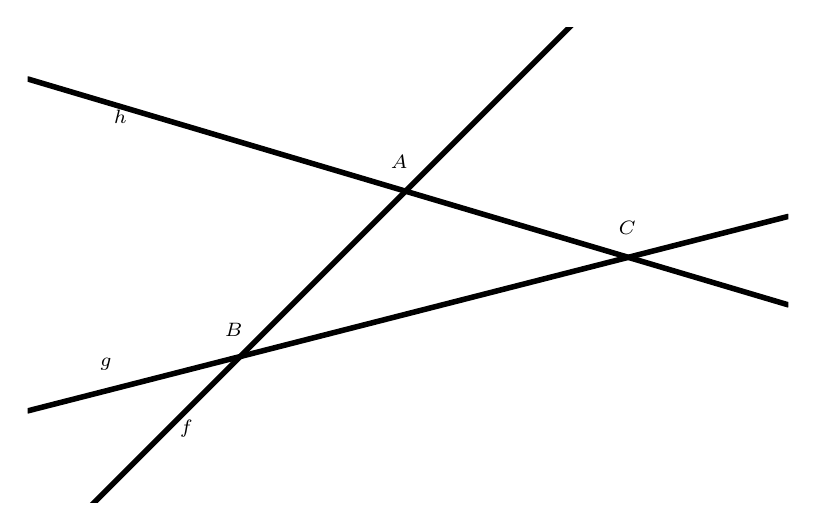
\begin{tikzpicture}[scale=0.7,line cap=round,line join=round,>=triangle 45,x=1cm,y=1cm]
\clip(-10.896666666666674,-1.4533333333333285) rectangle (2.9033333333333315,7.166666666666654);
\draw [line width=2pt,domain=-10.896666666666674:2.9033333333333315] plot(\x,{(-24.72-3*\x)/-3});
\draw [line width=2pt,domain=-10.896666666666674:2.9033333333333315] plot(\x,{(--21.12--1.8*\x)/7.04});
\draw [line width=2pt,domain=-10.896666666666674:2.9033333333333315] plot(\x,{(--12.12-1.2*\x)/4.04});
\begin{scriptsize}
\draw [color=black] (-4.04,4.2)-- ++(-0.5pt,-0.5pt) -- ++(1pt,1pt) ++(-1pt,0) -- ++(1pt,-1pt);
\draw[color=black] (-4.156666666666672,4.736666666666659) node {\textbf{$A$}};
\draw [color=black] (-7.04,1.2)-- ++(-0.5pt,-0.5pt) -- ++(1pt,1pt) ++(-1pt,0) -- ++(1pt,-1pt);
\draw[color=black] (-7.1566666666666725,1.6766666666666652) node {\textbf{$B$}};
\draw [color=black] (0,3)-- ++(-0.5pt,-0.5pt) -- ++(1pt,1pt) ++(-1pt,0) -- ++(1pt,-1pt);
\draw[color=black] (-0.016666666666669702,3.5366666666666613) node {\textbf{$C$}};
\draw[color=black] (-8.016666666666673,-0.10333333333333122) node {\textbf{$f$}};
\draw[color=black] (-9.476666666666674,1.0566666666666664) node {\textbf{$g$}};
\draw[color=black] (-9.216666666666674,5.556666666666657) node {\textbf{$h$}};
\end{scriptsize}
\end{tikzpicture}
\end{center}}
{1}
\end{exop}

\begin{resolu}{Alignés~?}
{En utilisant ta règle, complète les phrases suivantes par`` alignés'' ou ``non alignés'':
\begin{tasks}(2)
    \task $A,B$ et $C$ sont  non alignés.
    \task $B,C$ et $D$ sont alignés.
\end{tasks}
\begin{center}
	\includegraphics[scale=0.8]{media/es-11/13-r2}
%\psset{xunit=1cm,yunit=1cm,algebraic=true,dimen=middle,dotstyle=o,dotsize=5pt 0,linewidth=2pt,arrowsize=3pt 2,arrowinset=0.25}
%\begin{pspicture*}(-1.2344355704755743,-1.560808224779211)(4.60823592582183,4.6686122121714515)
%\psplot[linewidth=2pt,linecolor=blue]{-1.2344355704755743}{4.60823592582183}{(--1.3285142273184292-0.6906231083093861*x)/-0.37293647848706835}
%\begin{scriptsize}
%\psdots[dotstyle=x](-0.5852498486647523,2.5967428872432934)
%\rput[bl](-0.53,2.734867508905171){$A$}
%\psdots[dotstyle=x](3.2408021713692454,2.4448058034152287)
%\rput[bl](3.4203641795296864,2.4448058034152287){$B$}
%\psdots[dotstyle=x](2.923115541546928,1.8508699302691565)
%\rput[bl](3.0612401632088058,1.8370574681029688){$C$}
%\psdots[dotstyle=x](2.5501790630598595,1.1602468219597704)
%\rput[bl](2.7711784577188636,1.1049969732950193){$D$}
%\rput[bl](4.138612212171448,4.337113120182947){\blue}
%\end{scriptsize}
%\end{pspicture*}
\end{center}
}
{1}
\end{resolu}

\begin{exop}
{En utilisant ta règle, complète les phrases suivantes par ``alignés'' ou ``non alignés'':
%\psset{xunit=1cm,yunit=1cm,algebraic=true,dimen=middle,dotstyle=o,dotsize=5pt 0,linewidth=2pt,arrowsize=3pt 2,arrowinset=0.25}
%\begin{pspicture*}(-1.7700508240477888,-0.9148177659117839)(8.507825914091345,4.757333757241693)
%\begin{scriptsize}
%\psdots[dotstyle=x](-0.4333127648366866,2.707242584572795)
%\rput[bl](-0.37905998730715407,2.856312947029492){$A$}
%\psdots[dotstyle=x](-0.36360453356559175,1.8207975463447976)
%\rput[bl](-0.301782718599341,1.9753520837604237){$B$}
%\psdots[dotstyle=x](0.0639358731460712,1.5884331491115897)
%\rput[bl](0.130969986164412,1.7435202776369845){$C$}
%\psdots[dotstyle=x](0.6578717462921431,2.9420544413979863)
%\rput[bl](0.718277228343791,3.103600206894494){$D$}
%\psdots[dotstyle=x](2.1910550467389798,2.1271191735929107)
%\rput[bl](2.248367148758489,2.2844611585916756){$E$}
%\psdots[dotstyle=x](2.826428306383615,1.1049969732950193)
%\rput[bl](2.8820407521625557,1.2644012116485437){$F$}
%\psdots[dotstyle=x](2.743553533386488,3.0111167522289253)
%\rput[bl](2.804763483454743,3.1654220218607443){$G$}
%\psdots[dotstyle=x](1.8001589902531752,0.6925494232107272)
%\rput[bl](1.861980805219424,0.8471039606263533){$J$}
%\psdots[dotstyle=x](3.8711897916225664,0.1825194497391612)
%\rput[bl](3.933011606588813,0.33707398715478726){$K$}
%\psdots[dotstyle=x](0.23915816235535045,0.47617307082885074)
%\rput[bl](0.30097997732160064,0.6307276082444768){$M$}
%\psdots[dotstyle=x](2.2638226025000536,1.527143925255108)
%\rput[bl](2.325644417466302,1.681698462670734){$N$}
%\psdots[dotstyle=x](3.8093679766563158,3.134511114377619)
%\rput[bl](3.871189791622563,3.2890656517932455){$O$}
%\psdots[dotstyle=x](3.477837825442754,4.185971619518952)
%\rput[bl](3.546625263049748,4.340036506219502){$H$}
%\psdots[dotstyle=x](1.4910499154219228,2.068084806209799)
%\rput[bl](1.5528717303881718,2.2226393436254255){$I$}
%\psdots[dotstyle=x](5.239842648857282,-0.1545368509231192)
%\rput[bl](5.308546989587885,-0.00294599515959008){$L$}
%\end{scriptsize}
%\end{pspicture*}

\begin{tasks}(2)
    \task $A, C, D$ sont \ligne{4}
    \task $B, E, H$ sont \ligne{4}
    \task $G, H, K$ sont \ligne{4}
    \task $C, D, F$ sont \ligne{4}
    \task $A, I, M$ sont \ligne{4}
    \task $K, L, M$ sont \ligne{4}
    \task $B, I, K$ sont \ligne{4}
    \task $G, H, O$ sont \ligne{4}
\end{tasks}
\begin{center}
	\includegraphics[scale=1]{media/es-11/13-3}
\end{center}
}
{1}
\end{exop}

\begin{resolu}{Appartient?}{Après avoir observé la figure, complète avec les symboles $\in$ (appartient) ou $\notin$ (n'appartient pas).
\begin{tasks}(2)
    \task B \underline{\hspace{0.1cm} {\color{blue} $\in$}\hspace{0.1cm}} $(AD)$ 
    \task C \underline{\hspace{0.1cm}{\color{blue} $\notin$}\hspace{0.1cm}} $(AD)$
\end{tasks}
\begin{center}
	\includegraphics[scale=0.8]{media/es-11/13-r3}
\end{center}
%\psset{xunit=1cm,yunit=1cm,algebraic=true,dimen=middle,dotstyle=o,dotsize=5pt 0,linewidth=2pt,arrowsize=3pt 2,arrowinset=0.25}
%\begin{pspicture*}(-3.969209548684732,-2.011920033131499)(6.435346718365087,4.565167332297408)
%\psplot[linewidth=2pt]{-3.969209548684732}{6.435346718365087}{(--0.5960687340134798--1.3858077057592677*x)/1.4737954966011357}
%\begin{scriptsize}
%\psdots[dotstyle=x](-0.9556277123510664,-0.49413064110944277)
%\rput[bl](-0.867639921509204,0.1741611640047978){$A$}
%\psdots[dotstyle=x](0.5181677842500695,0.891677064649825)
%\rput[bl](0.6061555750919333,1.3116465417544703){$B$}
%\psdots[dotstyle=x](0.18821356859309876,2.8933993063021006)
%\rput[bl](0.27620135943496227,3.3133687834067465){$C$}
%\psdots[dotstyle=x](2.1717879382752265,2.4465736273898875)
%\rput[bl](2.2559266533767883,2.9734298291974548){$D$}
%\end{scriptsize}
%\end{pspicture*}
}
{1}
\end{resolu}

\begin{exop}
{Après avoir observé la figure, complète avec les symboles $\in$ (appartient) ou $\notin$ (n'appartient pas).
%\psset{xunit=1cm,yunit=1cm,algebraic=true,dimen=middle,dotstyle=o,dotsize=5pt 0,linewidth=2pt,arrowsize=3pt 2,arrowinset=0.25}
%\begin{pspicture*}(-2.6273957383463826,-1.1540390724233804)(7.777160528703436,5.423048293005525)
%\psplot[linewidth=2pt]{-2.6273957383463826}{7.777160528703436}{(--0.5960687340134798--1.3858077057592677*x)/1.4737954966011357}
%\begin{scriptsize}
%\psdots[dotstyle=x](-0.9556277123510664,-0.49413064110944277)
%\rput[bl](-0.867639921509204,0.17416116400479773){$A$}
%\psdots[dotstyle=x](0.5181677842500695,0.891677064649825)
%\rput[bl](0.6061555750919333,1.31164654175447){$B$}
%\psdots[dotstyle=x](2.849844241559336,3.069374887985817)
%\rput[bl](2.9378320324011953,3.4893443650904626){$C$}
%\psdots[dotstyle=x](3.751875141299478,3.932327266054473)
%\rput[bl](3.8397068885302494,4.347225325798581){$D$}
%\psdots[dotstyle=x](3.047816770953519,1.5515854959637614)
%\rput[bl](3.135804561795378,1.771554973068407){$E$}
%\psdots[dotstyle=x](2.607877816744224,4.543170384586943)
%\rput[bl](2.695865607586083,4.963139861691588){$F$}
%\end{scriptsize}
%\end{pspicture*}
\begin{tasks}(4)
    \task $B$ \ligne{1} $[CD)$
    \task $C$ \ligne{1} $(EF)$
    \task $C$ \ligne{1} $[AD]$
    \task $A$ \ligne{1} $[CE)$
\end{tasks}
\begin{center}
	\includegraphics[scale=0.8]{media/es-11/13-4}
\end{center}
}
{1}
\end{exop}

\begin{exop}
    {Indique par ``Vrai'' ou ``Faux'' si les droites suivantes sont perpendiculaires. 

	    \begin{minipage}[t]{0.4\textwidth}{
	    \vspace{0pt}
	    \begin{tasks}
	\task $f$ et $g$  \ligne{2}
    \task $f$ et $h$  \ligne{2}
    \task $i$ et $j$  \ligne{2}
    \task $h$ et $g$  \ligne{2}
    \task $i$ et $g$  \ligne{2}
    \task $j$ et $g$  \ligne{2}
\end{tasks}
	    }
	    \end{minipage}
	    \hfill
	    \begin{minipage}[t]{0.6\textwidth}{
	    \vspace{0pt}
\begin{center}
	\includegraphics[scale=0.8]{media/es-11/13-5}
\end{center}
	    }
	    \end{minipage}

%    \psset{xunit=1cm,yunit=1cm,algebraic=true,dimen=middle,dotstyle=o,dotsize=5pt 0,linewidth=2pt,arrowsize=3pt 2,arrowinset=0.25}
%\begin{pspicture*}(-4.66,-5.06)(9.1,1.68)
%\multips(0,-5)(0,1){7}{\psline[linestyle=dashed,linecap=1,dash=1.5pt 1.5pt,linewidth=0.4pt,linecolor=lightgray]{c-c}(-4.66,0)(9.1,0)}
%\multips(-4,0)(1,0){14}{\psline[linestyle=dashed,linecap=1,dash=1.5pt 1.5pt,linewidth=0.4pt,linecolor=lightgray]{c-c}(0,-5.06)(0,1.68)}
%\psplot[linewidth=2pt]{-4.66}{9.1}{(--2.62-2*x)/11}
%\psplot[linewidth=2pt]{-4.66}{9.1}{(-16--2*x)/12}
%\psplot[linewidth=2pt]{-4.66}{9.1}{(--64-11*x)/-2}
%\psplot[linewidth=2pt]{-4.66}{9.1}{(-13-6*x)/1}
%\psplot[linewidth=2pt]{-4.66}{9.1}{(-0-3*x)/3}
%\begin{scriptsize}
%\rput[bl](-4.5,1.2){$f$}
%\rput[bl](-4.5,-1.34){$g$}
%\rput[bl](5.7,1.2){$h$}
%\rput[bl](-2.16,1.2){$i$}
%\rput[bl](-0.98,1.2){$j$}
%\end{scriptsize}
%\end{pspicture*}

    }
    {1}
\end{exop}

\newpage
\begin{exop}
   {Complète avec les termes ``sécantes'' ou ``parallèles''.

	   \begin{minipage}[t]{0.45\textwidth}{
	   \vspace{0pt}	   
    \begin{tasks}
        \task $f$ et $i$ sont \ligne{3}
        \task $f$ et $h$ sont \ligne{3}
        \task $l$ et $k$ sont \ligne{3}
        \task $h$ et $k$ sont \ligne{3}
        \task $f$ et $j$ sont \ligne{3}
        \task $m$ et $k$ sont \ligne{3}
        \task $l$ et $i$ sont \ligne{3}
        \task $j$ et $i$ sont \ligne{3}
    \end{tasks}
	   }
	   \end{minipage}
	   \hfill
	   \begin{minipage}[t]{0.55\textwidth}{
	   \vspace{0pt}
\begin{center}
	\includegraphics[scale=0.7]{media/es-11/13-6}
\end{center}
	   }
	   \end{minipage}
%    \psset{xunit=1cm,yunit=1cm,algebraic=true,dimen=middle,dotstyle=o,dotsize=5pt 0,linewidth=2pt,arrowsize=3pt 2,arrowinset=0.25}
%\begin{pspicture*}(-4.66,-7.94)(10.3,1.68)
%\multips(0,-7)(0,1){10}{\psline[linestyle=dashed,linecap=1,dash=1.5pt 1.5pt,linewidth=0.4pt,linecolor=lightgray]{c-c}(-4.66,0)(10.3,0)}
%\multips(-4,0)(1,0){15}{\psline[linestyle=dashed,linecap=1,dash=1.5pt 1.5pt,linewidth=0.4pt,linecolor=lightgray]{c-c}(0,-7.94)(0,1.68)}
%\psplot[linewidth=2pt]{-4.66}{10.3}{(-6-2*x)/11}
%\psplot[linewidth=2pt]{-4.66}{10.3}{(-16--2*x)/12}
%\psplot[linewidth=2pt]{-4.66}{10.3}{(-43.12--2.18*x)/12.96}
%\psplot[linewidth=2pt]{-4.66}{10.3}{(-48.84-0.98*x)/14.66}
%\psplot[linewidth=2pt]{-4.66}{10.3}{(-61-2*x)/11}
%\psline[linewidth=2pt](3,-7.94)(3,1.68)
%\psline[linewidth=2pt](-2,-7.94)(-2,1.68)
%\psplot[linewidth=2pt]{-4.66}{10.3}{(--38-8*x)/-10}
%\begin{scriptsize}
%\rput[bl](-4.5,0.48){$f$}
%\rput[bl](-4.5,-1.82){$g$}
%\rput[bl](-4.5,-3.92){$h$}
%\rput[bl](-4.5,-2.82){$i$}
%\rput[bl](-4.5,-4.56){$j$}
%\rput[bl](2.66,1.2){$k$}
%\rput[bl](-1.84,1.2){$l$}
%\rput[bl](-4.5,-6.94){$m$}
%\end{scriptsize}
%\end{pspicture*}
    }
    {1}
\end{exop}

\begin{exof}{ES1}{106}{1}
\end{exof}


\begin{exop}
    {Complète avec les symboles $\paral$, $\perp$ ou laisse vide si aucun ne convient.

	    \begin{minipage}[t]{0.3\textwidth}{
	    \vspace{0pt}
	        \begin{tasks}
        \task $c$ \ligne{2} $b$
        \task $f$ \ligne{2} $c$
        \task $d$ \ligne{2} $b$
        \task $a$ \ligne{2} $e$
        \task $d$ \ligne{2} $e$
        \task $c$ \ligne{2} $a$
    \end{tasks}
	    }
	    \end{minipage}
	    \begin{minipage}[t]{0.7\textwidth}{
	    \vspace{0pt}
 \begin{center}
	    \includegraphics[scale=0.7]{media/es-11/13-7}
%    \psset{xunit=1cm,yunit=1cm,algebraic=true,dimen=middle,dotstyle=o,dotsize=5pt 0,linewidth=2pt,arrowsize=3pt 2,arrowinset=0.25}
%\begin{pspicture*}(-4.1,-3.37)(5.2,3.37)
%\multips(0,-3)(0,1){7}{\psline[linestyle=dashed,linecap=1,dash=1.5pt 1.5pt,linewidth=0.4pt,linecolor=lightgray]{c-c}(-4.1,0)(5.2,0)}
%\multips(-4,0)(1,0){10}{\psline[linestyle=dashed,linecap=1,dash=1.5pt 1.5pt,linewidth=0.4pt,linecolor=lightgray]{c-c}(0,-3.37)(0,3.37)}
%\psline[linewidth=2pt](-4,-1)(0,2)
%\psline[linewidth=2pt](0,2)(2,-1)
%\psline[linewidth=2pt](2,-1)(-4,-1)
%\psline[linewidth=2pt](-3.68,0.99)(0.6723076923076924,0.9915384615384615)
%\psplot[linewidth=2pt]{-4.1}{5.2}{(--1.63--2*x)/3}
%\psplot[linewidth=2pt]{-4.1}{5.2}{(--107.34--36*x)/-24}
%\begin{scriptsize}
%\psdots[dotstyle=x](0,2)
%\rput[bl](0.08,2.19){$A$}
%\psdots[dotstyle=x](-4,-1)
%\rput[bl](-3.92,-0.81){$B$}
%\psdots[dotstyle=x](2,-1)
%\rput[bl](2.08,-0.81){$C$}
%\psdots[dotstyle=x](-3.68,0.99)
%\rput[bl](-3.6,1.19){$D$}
%\psdots[dotstyle=x](0.6723076923076924,0.9915384615384615)
%\rput[bl](0.76,1.19){$E$}
%\psdots[dotsize=4pt 0,dotstyle=x,linecolor=darkgray](-2.315,-1)
%\rput[bl](-2.24,-0.85){\darkgray{$F$}}
%\end{scriptsize}
%\end{pspicture*}
  \end{center} 
	    }
	    \end{minipage} 
       }
    {1}
\end{exop}


%\begin{resolu}{Traçons des perpendiculaires}{Construis la droite $d2$ perpendiculaire à la droite $d1$ passant par $A$.
%\psset{xunit=1cm,yunit=1cm,algebraic=true,dimen=middle,dotstyle=o,dotsize=5pt 0,linewidth=2pt,arrowsize=3pt 2,arrowinset=0.25}
%\begin{pspicture*}(-4.1,-1.95)(4.82,3.37)
%\multips(0,-1)(0,1){6}{\psline[linestyle=dashed,linecap=1,dash=1.5pt 1.5pt,linewidth=0.4pt,linecolor=lightgray]{c-c}(-4.1,0)(4.82,0)}
%\multips(-4,0)(1,0){9}{\psline[linestyle=dashed,linecap=1,dash=1.5pt 1.5pt,linewidth=0.4pt,linecolor=lightgray]{c-c}(0,-1.95)(0,3.37)}
%\psline[linewidth=2pt](0,-1.95)(0,3.37)
%\psline[linewidth=2pt,linestyle=dotted](-3,1)(0,1)
%\begin{scriptsize}
%\rput[bl](0.14,2.89){$d1$}
%\psdots[dotstyle=x](-3,1)
%\rput[bl](-2.92,1.21){$A$}
%\end{scriptsize}
%\end{pspicture*}
%{\color{blue} A l'aide de l'équerre, trace le segment perpendiculaire à la droite d1 passant par A. Il faut aligner un des deux cotés de l'équerre formant un angle droit avec d1 et que l'autre passe par le point A.}
%}
%{1}
%\end{resolu}

\begin{exop}{Construis la droite 
		\begin{tasks}[after-item-skip = 0.4em](2)
	\task $d' \perp d$ passant par le point $A$.
	\task $d''\perp d$ passant par le point $B$.
	\task $e'\perp e$ passant par le point $A$.
	\task $e''\perp e$ passant par le point $B$.
\end{tasks}
	
\begin{center}
	\includegraphics[scale=0.8]{media/es-11/13-8}
%\psset{xunit=1cm,yunit=1cm,algebraic=true,dimen=middle,dotstyle=o,dotsize=5pt 0,linewidth=2pt,arrowsize=3pt 2,arrowinset=0.25}
%\begin{pspicture*}(-4.1,-1.77)(16.96,3.37)
%\psline[linewidth=2pt](0,-1.77)(0,3.37)
%\psline[linewidth=2pt](9,-1.77)(10.5,3.37)
%\begin{scriptsize}
%\rput[bl](-0.44,2.75){$d1$}
%\psdots[dotstyle=x](-3,1)
%\rput[bl](-2.92,1.21){$A$}
%\rput[bl](9.9,2.89){$d1$}
%\psdots[dotstyle=x](8.64,-0.01)
%\rput[bl](8.72,0.19){$A$}
%\end{scriptsize}
%\end{pspicture*}
\end{center}}
{1}
\end{exop}

\begin{exop}{Construis la droite
		\begin{tasks}[after-item-skip = 0.4em](2)
	\task $d' \perp d$ passant par le point $A$.
	\task $d''\perp d$ passant par le point $B$.
	\task $e'\perp e$ passant par le point $A$.
	\task $e''\perp e$ passant par le point $B$.
\end{tasks}
	
\begin{center}
\includegraphics[scale=0.8]{media/es-11/13-9}
%\psset{xunit=1cm,yunit=1cm,algebraic=true,dimen=middle,dotstyle=o,dotsize=5pt 0,linewidth=2pt,arrowsize=3pt 2,arrowinset=0.25}
%\begin{pspicture*}(-4.1,-1.77)(16.96,3.37)
%\psline[linewidth=2pt](0,-1.77)(0,3.37)
%\psline[linewidth=2pt](9,-1.77)(10.5,3.37)
%\begin{scriptsize}
%\rput[bl](-0.44,2.75){$d1$}
%\psdots[dotstyle=x](-3,1)
%\rput[bl](-2.92,1.21){$A$}
%\rput[bl](9.9,2.89){$d1$}
%\psdots[dotstyle=x](8.64,-0.01)
%\rput[bl](8.72,0.19){$A$}
%\end{scriptsize}
%\end{pspicture*}
\end{center}}
{1}
\end{exop}


 %\begin{resolu}{Traçons des parallèles}{Construis la droite d2 parallèle à la droite d1 passant par A.
%\psset{xunit=1cm,yunit=1cm,algebraic=true,dimen=middle,dotstyle=o,dotsize=5pt 0,linewidth=2pt,arrowsize=3pt 2,arrowinset=0.25}
%\begin{pspicture*}(-4.1,-1.95)(4.82,3.37)
%\multips(0,-1)(0,1){6}{\psline[linestyle=dashed,linecap=1,dash=1.5pt 1.5pt,linewidth=0.4pt,linecolor=lightgray]{c-c}(-4.1,0)(4.82,0)}
%\multips(-4,0)(1,0){9}{\psline[linestyle=dashed,linecap=1,dash=1.5pt 1.5pt,linewidth=0.4pt,linecolor=lightgray]{c-c}(0,-1.95)(0,3.37)}
%\psline[linewidth=2pt](0,-1.95)(0,3.37)
%\psline[linewidth=2pt,linestyle=dotted](-3,1)(0,1)
%\psline[linewidth=1.2pt,linestyle=dashed,dash=1pt 1pt](-3,-1.95)(-3,3.37)
%\begin{scriptsize}
%\rput[bl](0.14,2.89){$d1$}
%\psdots[dotstyle=x](-3,1)
%\rput[bl](-2.92,1.21){$A$}
%\end{scriptsize}
%\end{pspicture*}
%{\color{blue} A l'aide de l'équerre, trace le segment perpendiculaire à la droite d1 passant par A. Puis, trace la droite perpendiculaire à ce segment.}
%}
%{1}
%\end{resolu}

\begin{exop}{Construis la droite
\begin{tasks}[after-item-skip = 0.4em](2)
	\task $d'\paral d$ passant par le point $A$.
	\task  $d''\paral d$ passant par le point $B$.
	\task  $e'\paral e$ passant par le point $A$.
	\task  $e''\paral e$ passant par le point $B$.
\end{tasks}
	
\begin{center}
\includegraphics[scale=0.8]{media/es-11/13-8}
\end{center}
%    \psset{xunit=1cm,yunit=1cm,algebraic=true,dimen=middle,dotstyle=o,dotsize=5pt 0,linewidth=2pt,arrowsize=3pt 2,arrowinset=0.25}
%\begin{pspicture*}(-4.1,-1.77)(16.96,3.37)
%\psline[linewidth=2pt](0,-1.77)(1,3.37)
%\psline[linewidth=1.2pt](9,-1.77)(9,3.37)
%\begin{scriptsize}
%\rput[bl](1,2.75){$d1$}
%\psdots[dotstyle=x](-3,1)
%\rput[bl](-2.92,1.21){$A$}
%\rput[bl](8.66,2.89){$d1$}
%\psdots[dotstyle=x](8.64,-0.01)
%\rput[bl](8.72,0.19){$A$}
%\end{scriptsize}
%\end{pspicture*}
    }{1}
\end{exop}


\begin{exop}{Construis la droite 
\begin{tasks}[after-item-skip = 0.4em](2)
	\task  $d'\paral d$ passant par le point $A$.
	\task  $d''\paral d$ passant par le point $B$.
	\task  $e'\paral e$ passant par le point $A$.
	\task  $e''\paral e$ passant par le point $B$.
\end{tasks}
	
\begin{center}
\includegraphics[scale=0.8]{media/es-11/13-9}
\end{center}
    }{1}
\end{exop}

\begin{exol}{ES9}{97}{1}
\end{exol}
\begin{resolu}{Mesures}{Mesure la longueur du segment ci-dessous:

\begin{center}
  
\includegraphics[scale=0.5]{media/es-11/regleseg}  
\end{center}
{\color{blue} Le segment mesure 5,2 cm.}
}
{1}
\end{resolu}

\begin{exop}
{Mesure la longueur des segments suivants:
%\begin{center}
%\psset{xunit=1cm,yunit=1cm,algebraic=true,dimen=middle,dotstyle=o,dotsize=5pt 0,linewidth=2pt,arrowsize=3pt 2,arrowinset=0.25}
%\begin{pspicture*}(-3.969209548684732,-3.7056850068372698)(9.25095602530456,4.565167332297408)
%\psline[linewidth=2pt](-2,2)(2,2)
%\psline[linewidth=2pt](-2,1)(4,1)
%\psline[linewidth=2pt](-2,0)(5,0)
%\psline[linewidth=2pt](-2,-1)(1.5080304312209643,-0.9560665430291987)
%\psline[linewidth=2pt](-2,-2)(-1,-2)
%\psline[linewidth=2pt](-2,-3)(0,-3)
%\begin{scriptsize}
%\psdots[dotstyle=x](-2,2)
%\rput[bl](-2.1654598364266255,2.431463404382345){$A$}
%\psdots[dotstyle=x](2,2)
%\rput[bl](1.947969385430276,2.431463404382345){$B$}
%\psdots[dotstyle=x](-2,1)
%\rput[bl](-2.143462888716161,1.3756099142800455){$C$}
%\psdots[dotstyle=x](4,1)
%\rput[bl](3.9056977316616353,1.507591600542833){$D$}
%\psdots[dotstyle=x](-2,0)
%\rput[bl](-1.901496463901049,0.2097716856254234){$E$}
%\psdots[dotstyle=x](5,0)
%\rput[bl](5.09353290802673,0.2097716856254234){$F$}
%\psdots[dotstyle=x](-2,-1)
%\rput[bl](-1.901496463901049,-0.7800909613454822){$G$}
%\psdots[dotstyle=x](1.5080304312209643,-0.9560665430291987)
%\rput[bl](1.5960182220628405,-0.736097065924553){$H$}
%\psdots[dotstyle=x](-2,-2)
%\rput[bl](-1.901496463901049,-1.7699536083163878){$I$}
%\psdots[dotstyle=x](-1,-2)
%\rput[bl](-0.9116338169301369,-1.7699536083163878){$J$}
%\psdots[dotstyle=x](-2,-3)
%\rput[bl](-1.901496463901049,-2.781813202997758){$K$}
%\psdots[dotstyle=x](0,-3)
%\rput[bl](0.0782288300407752,-2.781813202997758){$L$}
%\end{scriptsize}
%\end{pspicture*}
%\end{center}

\begin{minipage}[t]{0.3\textwidth}{
\vspace{0pt}
\begin{tasks}
     \task $AB=$ \ligne{1.5}cm
     \task $CD=$  \ligne{1.5}cm
     \task $EF=$  \ligne{1.5}cm
     \task $GH=$  \ligne{1.5}cm
     \task $IJ=$ \ligne{1.5}cm
     \task $KL=$  \ligne{1.5}cm     
\end{tasks}
}
\end{minipage}
\begin{minipage}[t]{0.7\textwidth}{
\vspace{0pt}
\begin{center}
\includegraphics[scale=0.7]{media/es-11/13-12}
\end{center}
}
\end{minipage}
}
{1}
\end{exop}

\newpage
\begin{exop}
{Sur les demi-droites ci-dessous, place les points B, D et F tels que:
\begin{tasks}(3)
    \task $AB=5$ cm
    \task $CD=3,6$ cm
    \task $EF=4,3$ cm
\end{tasks}
\begin{center}
\includegraphics[scale=0.8]{media/es-11/13-13}
\end{center}
%\psset{xunit=1cm,yunit=1cm,algebraic=true,dimen=middle,dotstyle=o,dotsize=5pt 0,linewidth=2pt,arrowsize=3pt 2,arrowinset=0.25}
%\begin{pspicture*}(-2.6273957383463826,0.14378084249402764)(13.078424926925438,3.839268057852087)
%\psplot[linewidth=2pt]{-2}{13.078424926925438}{(--21-0*x)/7}
%\psplot[linewidth=2pt]{-2}{13.078424926925438}{(--20-0*x)/10}
%\psplot[linewidth=2pt]{-2}{13.078424926925438}{(--11-0*x)/11}
%\begin{scriptsize}
%\psdots[dotstyle=x](-2,3)
%\rput[bl](-1.901496463901046,3.2233535219590768){$A$}
%\psdots[dotstyle=x](-2,2)
%\rput[bl](-1.901496463901046,2.2114939272777034){$C$}
%\psdots[dotstyle=x](-2,1)
%\rput[bl](-1.901496463901046,1.2216312803067946){$E$}
%\end{scriptsize}
%\end{pspicture*}
}    
{1}
\end{exop}

%\begin{resolu}{Distances}{Mesure la distance des points $A$ et $B$ à la droite $d$:
%
%\begin{tasks}
%    \task Distance A à d:{\color{blue} 1,9} cm
%    \task Distance B à d:{\color{blue} 1,4} cm
%\end{tasks}
%
%{\color{blue} La distance la plus courte se mesure en traçant les droites perpendiculaires à d passant par A et B.}
%
%\begin{center}
%
%\psset{xunit=1cm,yunit=1cm,algebraic=true,dimen=middle,dotstyle=o,dotsize=5pt 0,linewidth=2pt,arrowsize=3pt 2,arrowinset=0.25}
%\begin{pspicture*}(-6.73,-2.57)(6.71,2.57)
%\psplot[linewidth=2pt]{-6.73}{6.71}{(-2.3356--0.98*x)/3.38}
%\psplot[linewidth=2pt]{-6.73}{6.71}{(--2.4--3.38*x)/-0.98}
%\psplot[linewidth=2pt]{-6.73}{6.71}{(-12.54--3.38*x)/-0.98}
%\psline[linewidth=2pt](3.607170725405336,0.35486015115302627)(4,-1)
%\begin{scriptsize}
%\rput[bl](-5.03,-2.01){$d$}
%\psdots[dotstyle=x](-1,1)
%\rput[bl](-0.93,1.19){$A$}
%\psdots[dotstyle=x](4,-1)
%\rput[bl](4.07,-0.81){$B$}
%\end{scriptsize}
%\end{pspicture*}
%\end{center}}
%{1}
%\end{resolu}

\begin{exop}
{Mesure la distance des points $A$, $B$, $C$ et $D$ à la droite $d$:

	\begin{minipage}[t]{0.5\textwidth}{
	\vspace{0pt}	
\begin{tasks}
    \task Distance de $A$ à $d=$\ligne{1.5}cm
    \task Distance de $B$ à $d=$\ligne{1.5}cm
    \task Distance de $C$ à $d=$\ligne{1.5}cm
    \task Distance de $D$ à $d=$\ligne{1.5}cm
\end{tasks}
	}
	\end{minipage}
	\begin{minipage}[t]{0.5\textwidth}{
	\vspace{0pt}
\begin{center}
\includegraphics[scale=0.7]{media/es-11/13-14}
\end{center}	}
	\end{minipage}
%\psset{xunit=1cm,yunit=1cm,algebraic=true,dimen=middle,dotstyle=o,dotsize=5pt 0,linewidth=2pt,arrowsize=3pt 2,arrowinset=0.25}
%\begin{pspicture*}(-10.97,-4.65)(-0.35,2.87)
%\psplot[linewidth=2pt]{-10.97}{-0.35}{(--3--1*x)/2}
%\begin{scriptsize}
%\rput[bl](-9.27,-3.69){$d$}
%\psdots[dotstyle=x](-7,-1)
%\rput[bl](-6.91,-0.79){$A$}
%\psdots[dotstyle=x](-5,-4)
%\rput[bl](-4.91,-3.79){$B$}
%\psdots[dotstyle=x](-4.99,0.43)
%\rput[bl](-4.91,0.63){$C$}
%\psdots[dotstyle=x](-3.01,-2.77)
%\rput[bl](-2.93,-2.57){$D$}
%\end{scriptsize}
%\end{pspicture*}
}
{1}
\end{exop}

\newpage
\begin{exop}
{
Quelles sont les distances du point $A$ aux droites $d1, d2, d3, d4, d5$ et $d6$~? 

\begin{minipage}[t]{0.47\textwidth}{
\vspace{0pt}
\begin{tasks}
    \task Distance $A$ à $d1=$\ligne{1.5}cm
    \task Distance $A$ à $d2=$\ligne{1.5}cm
    \task Distance $A$ à $d3=$\ligne{1.5}cm
    \task Distance $A$ à $d4=$\ligne{1.5}cm
    \task Distance $A$ à $d5=$\ligne{1.5}cm
    \task Distance $A$ à $d6=$\ligne{1.5}cm
\end{tasks}
}
\end{minipage}
\begin{minipage}[t]{0.53\textwidth}{
\vspace{0pt}
\begin{center}
\includegraphics[scale=0.8]{media/es-11/13-15}
\end{center}	
}
\end{minipage}
%\psset{xunit=1cm,yunit=1cm,algebraic=true,dimen=middle,dotstyle=o,dotsize=5pt 0,linewidth=2pt,arrowsize=3pt 2,arrowinset=0.25}
%\begin{pspicture*}(-11.39,-4.87)(-0.77,2.65)
%\psplot[linewidth=2pt]{-11.39}{-0.77}{(-27.7318-4.98*x)/2.48}
%\psplot[linewidth=2pt]{-11.39}{-0.77}{(-9.844-3.02*x)/3.66}
%\psplot[linewidth=2pt]{-11.39}{-0.77}{(-15.1292-2.76*x)/-1.36}
%\psplot[linewidth=2pt]{-11.39}{-0.77}{(--25.939--2.84*x)/3.1}
%\psplot[linewidth=2pt]{-11.39}{-0.77}{(-34.9658-3.28*x)/5.5}
%\psplot[linewidth=2pt]{-11.39}{-0.77}{(--19.7754--4.6*x)/5.98}
%\begin{scriptsize}
%\psdots[dotstyle=x](-6.97,-0.03)
%\rput[bl](-7.17,0.27){$A$}
%\rput[bl](-7.23,2.17){$d1$}
%\rput[bl](-6.01,1.61){$d2$}
%\rput[bl](-4.81,2.17){$d3$}
%\rput[bl](-11.23,-1.35){$d5$}
%\rput[bl](-11.21,0.65){$d6$}
%\rput[bl](-9.35,-3.53){$d4$}
%\end{scriptsize}
%\end{pspicture*}
}
{1}
\end{exop}

%\begin{resolu}{Distances}{Soient f et g, deux droites parallèles. Donne la distance qui sépare les droites f et g:
%
%\begin{center}
%\psset{xunit=1cm,yunit=1cm,algebraic=true,dimen=middle,dotstyle=o,dotsize=5pt 0,linewidth=2pt,arrowsize=3pt 2,arrowinset=0.25}
%\begin{pspicture*}(-10.97,-4.65)(-0.35,2.87)
%\psplot[linewidth=2pt]{-10.97}{-0.35}{(--13--2*x)/5}
%\psplot[linewidth=2pt]{-10.97}{-0.35}{(--3--2*x)/5}
%\psplot[linewidth=2pt]{-10.97}{-0.35}{(--29.65--5*x)/-2}
%\begin{scriptsize}
%\rput[bl](-10.81,-1.53){$f$}
%\rput[bl](-10.81,-3.53){$g$}
%\rput[bl](-6.99,1.65){$h$}
%\end{scriptsize}
%\end{pspicture*}
%\end{center}
%{\color{blue} La distance la plus courte entre deux droites parallèles est le segment perpendiculaire entre ces deux droites.}
% Distance de f à g:{\color{blue} 1,9} cm.}
%{1}
%\end{resolu}

\newpage
\begin{exop}
{Sachant que $f\paral i$ et $g\paral h$, mesure les distances demandées:
\begin{tasks}(2)
    \task Distance de $f$ à $i =$\ligne{1.5}cm
     \task Distance de $g$ à $h =$\ligne{1.5}cm
\end{tasks}
\begin{center}
\includegraphics[scale=0.8]{media/es-11/13-16}
\end{center}	
%\psset{xunit=1cm,yunit=1cm,algebraic=true,dimen=middle,dotstyle=o,dotsize=5pt 0,linewidth=2pt,arrowsize=3pt 2,arrowinset=0.25}
%\begin{pspicture*}(-10.97,-6.13)(5.11,2.87)
%\psplot[linewidth=2pt]{-10.97}{5.11}{(--2-1*x)/6}
%\psplot[linewidth=2pt]{-10.97}{5.11}{(--3--2*x)/5}
%\psplot[linewidth=2pt]{-10.97}{5.11}{(--7-2*x)/-5}
%\psplot[linewidth=2pt]{-10.97}{5.11}{(-10-1*x)/6}
%\begin{scriptsize}
%\rput[bl](-10.81,2.39){$f$}
%\rput[bl](-10.81,-3.53){$g$}
%\rput[bl](-10.81,-5.53){$h$}
%\rput[bl](-10.81,0.33){$i$}
%\end{scriptsize}
%\end{pspicture*}
}
{1}
\end{exop}

\begin{exof}{ES3}{107}{1}
\end{exof}

\begin{exof}{ES7}{109}{1}
\end{exof}

\begin{exof}{ES8}{109}{1}
\end{exof}

\begin{exop}
{Place le point $A$ à \tunit{1,2}{\cm} de la droite $d$. Y-a-t-il qu'une seule solution possible pour placer ce point~? Quelle(s) figure(s) géométrique(s) représente(nt) tous les lieux où ce point peut être placé~?


\begin{center}
\includegraphics[scale=0.8]{media/es-11/13-17}
\end{center}	
%\psset{xunit=1cm,yunit=1cm,algebraic=true,dimen=middle,dotstyle=o,dotsize=5pt 0,linewidth=2pt,arrowsize=3pt 2,arrowinset=0.25}
%\begin{pspicture*}(-3.63,-4.22)(9.99,1.3)
%\psplot[linewidth=2pt]{-3.63}{9.99}{(-14.5524-1.48*x)/9.5}
%\begin{scriptsize}
%\rput[bl](-2.87,-0.8){$d$}
%\end{scriptsize}
%\end{pspicture*}
}
{2}
\end{exop}
\end{document}
